% MICCAI 2026 -- MRIxFields Task 3, team inzva_mri. Five minutes, seven slides.
% Compile from inside reports/:  ~/anaconda3/envs/tex/bin/tectonic slides_miccai.tex
%
% Numbers: every SSIM/nRMSE is a *challenge* score off the Task 3 leaderboard
% (syn74915588, pulled 2026-09-14), same table reports/architecture_report.tex uses.
% Spectral alphas: reports/spectral/alpha_summary.csv, retrospective split, 30 volumes
% per cell. Per-field error: reports/error_by_field.tex. Qualitative panel:
% scripts/make_slides_qualitative.py, shipped weights, TTA on.
%
% Logos: drop itu.pdf / itu.png and inzva.pdf / inzva.png into reports/logos/ and they
% are picked up automatically; until then a plain wordmark stands in, so the deck always
% compiles.
\documentclass[aspectratio=169,11pt]{beamer}

\usetheme{default}
\usepackage{lmodern}
\usepackage[T1]{fontenc}
\usepackage{amsmath}
\usepackage{booktabs}
\usepackage{graphicx}
\usepackage{tikz}
\usetikzlibrary{positioning,arrows.meta}

\setbeamertemplate{navigation symbols}{}
\setbeamertemplate{footline}[frame number]
\setbeamercolor{frametitle}{fg=black}
\setbeamercolor{structure}{fg=black!70}
\setbeamerfont{frametitle}{size=\large,series=\bfseries}
\setbeamertemplate{itemize item}{\textbf{--}}

% Same palette as reports/architecture_report.tex, so the deck and the report read as
% one document: red = what changed, blue = information added, grey = dropped.
\definecolor{accent}{HTML}{D64545}
\definecolor{cond}{HTML}{3E7CB1}
\definecolor{ink}{HTML}{102A43}
\definecolor{muted}{HTML}{627D98}
\definecolor{baseline}{HTML}{D9E2EC}
\definecolor{keep}{HTML}{2F6B3A}

\newcommand{\hl}[1]{\textcolor{accent}{\textbf{#1}}}
\newcommand{\info}[1]{\textcolor{cond}{\textbf{#1}}}
\newcommand{\gloss}[1]{{\footnotesize\textcolor{black!65}{#1}}\par}
\newcommand{\srcline}[1]{\vfill{\scriptsize\textcolor{gray}{#1}}}

% The logos we were given are white artwork on transparency, invisible on a light
% slide, so logos/*_dark.png are the same files with RGB inverted and alpha untouched.
% Each slot takes the first file that exists, so dropping an official colour version in
% picks it up with no edit here:
%     logos/<name>.pdf  ->  <name>.png  ->  plain wordmark
% ITU is the official black original (itu_logo_siyah.png), not a recolour: their brand
% guidance wants the supplied artwork. inzva is white-on-transparent, so inzva_logo_dark
% is that file with RGB inverted and alpha untouched.
\newcommand{\logoslot}[3]{%
  \IfFileExists{logos/#1.pdf}{\includegraphics[height=#3]{logos/#1.pdf}}{%
  \IfFileExists{logos/#1.png}{\includegraphics[height=#3]{logos/#1.png}}{%
    \raisebox{0.15\height}{\fbox{\rule{0pt}{#3}\,\textsf{\textbf{#2}}\,}}}}}

\begin{document}

% ==================================================================== 1. title
\begin{frame}[plain]
  \vfill
  \centering
  {\Large\bfseries Two problems wearing one metric}\\[1.5mm]
  {\large Cross-field brain MRI translation, MRIxFields 2026 Task 3}\\[5mm]

  {\small Berkin Deniz Kahya\textsuperscript{1,2} \quad
          Racha Badreddine\textsuperscript{1,2} \quad
          Furkan Y\"uceyal\c{c}\i n\textsuperscript{2} \quad
          Ahmet Zelka\textsuperscript{2}}\\[2mm]
  {\footnotesize\textcolor{muted}{%
    \textsuperscript{1}\.Istanbul Technical University, PIMI Lab \quad
    \textsuperscript{2}inzva}}\\[6mm]

  \logoslot{itu_logo_siyah}{\.ITU}{12mm}\hspace{16mm}%
  \raisebox{2.2mm}{\logoslot{inzva_logo_dark}{inzva}{7mm}}\\[6mm]

  {\footnotesize Team \texttt{inzva\_mri} \;\textbf{$\cdot$}\; final SSIM \hl{0.913652}}
  \vfill
\end{frame}

% ================================================================= 2. the task
\begin{frame}{The task, and the number to beat}
  \begin{columns}[c,onlytextwidth]
  \begin{column}{0.46\textwidth}
    \centering
    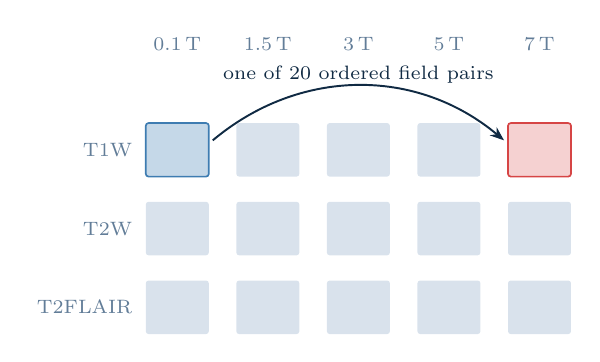
\begin{tikzpicture}[x=1cm,y=1cm,font=\scriptsize]
      \foreach \c/\f in {0/0.1\,T,1/1.5\,T,2/3\,T,3/5\,T,4/7\,T}{
        \node[text=muted] at (\c*1.15,1.35) {\f};}
      \foreach \r/\m in {0/T1W,1/T2W,2/T2FLAIR}{
        \node[text=muted,anchor=east] at (-0.45,-\r*1.0) {\m};
        \foreach \c in {0,1,2,3,4}{
          \fill[fill=baseline,rounded corners=1pt]
            (\c*1.15-0.4,-\r*1.0-0.34) rectangle ++(0.8,0.68);}}
      \fill[cond!30,draw=cond,rounded corners=1pt,line width=0.6pt]
        (-0.4,-0.34) rectangle ++(0.8,0.68);
      \fill[accent!25,draw=accent,rounded corners=1pt,line width=0.6pt]
        (4*1.15-0.4,-0.34) rectangle ++(0.8,0.68);
      \draw[->,draw=ink,line width=0.7pt,>={Stealth[length=1.8mm]}]
        (0.45,0.12) to[out=40,in=140] (4*1.15-0.45,0.12);
      \node[text=ink] at (2.3,0.95) {one of 20 ordered field pairs};
    \end{tikzpicture}

    \vspace{3mm}
    \gloss{15 domains $=$ 3 modalities $\times$ 5 fields.}
  \end{column}

  \begin{column}{0.5\textwidth}
    \textbf{Submission: copy the input, $\hat y = x$.}

    \vspace{4mm}
    \centering
    \begin{tabular}{lcc}
      \toprule
      & SSIM & nRMSE \\
      \midrule
      $\hat y = x$      & \hl{0.836497} & 0.5216 \\
      our final model   & \hl{0.913652} & 0.2380 \\
      \bottomrule
    \end{tabular}

    \vspace{4mm}
    \raggedright
    \gloss{Our whole gain over copying: \hl{$+0.0772$}.}
  \end{column}
  \end{columns}
\end{frame}

% =========================================================== 3. spectral, why
\begin{frame}{Before modelling: what is actually missing?}
  \centering
  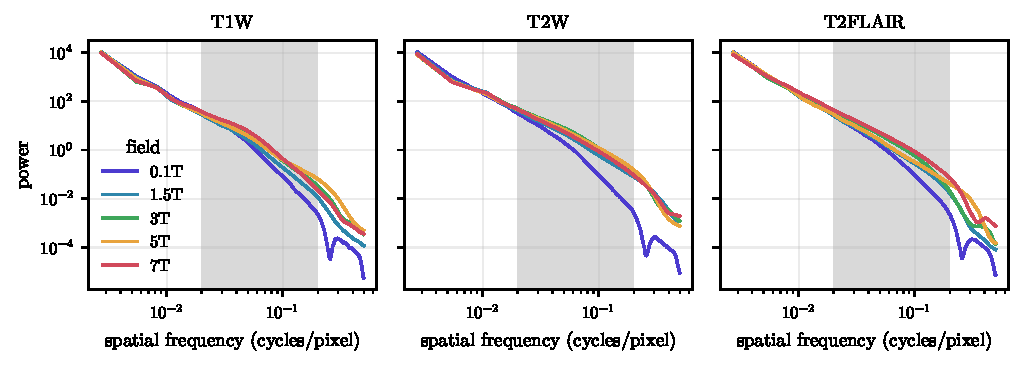
\includegraphics[width=0.90\textwidth]{spectral/fig_rapsd_by_field_retro.pdf}

  \vspace{-1mm}
  \begin{columns}[t,onlytextwidth]
  \begin{column}{0.53\textwidth}
    \centering\scriptsize
    \setlength{\tabcolsep}{3.5pt}
    fitted slope $\alpha$, \emph{minus} the 7\,T target's\par
    \vspace{0.6mm}
    \begin{tabular}{lcccc}
      \toprule
       & 0.1\,T & 1.5\,T & 3\,T & 5\,T \\
      \midrule
      T1W     & \hl{$+1.01$} & $+0.16$ & $-0.17$ & \info{$-0.51$} \\
      T2W     & \hl{$+1.50$} & $+0.10$ & $-0.06$ & \info{$-0.21$} \\
      T2FLAIR & \hl{$+1.29$} & $+0.35$ & $+0.34$ & $+0.18$ \\
      \bottomrule
    \end{tabular}
  \end{column}
  \begin{column}{0.45\textwidth}
    \footnotesize
    \begin{itemize}\setlength{\itemsep}{1.2mm}
      \item \hl{Positive: never acquired.} 0.1\,T holds ${\sim}3\%$ of 7\,T's fine
            detail. It has to be \emph{generated}.
      \item \info{Negative: too much detail.} 3\,T and 5\,T are finer than 7\,T. The
            right map is a \emph{blur}.
    \end{itemize}
  \end{column}
  \end{columns}

  \vspace{1.5mm}
  {\scriptsize\textcolor{gray}{Radially averaged power spectral density,
  $P(f)\propto f^{-\alpha}$, fitted on 0.02--0.2 cycles/pixel, 30 volumes per cell.}\par}
\end{frame}

% ================================================= 4. the prediction held up
\begin{frame}{The split is where the error goes}
  \begin{columns}[c,onlytextwidth]
  \begin{column}{0.52\textwidth}
    \centering
    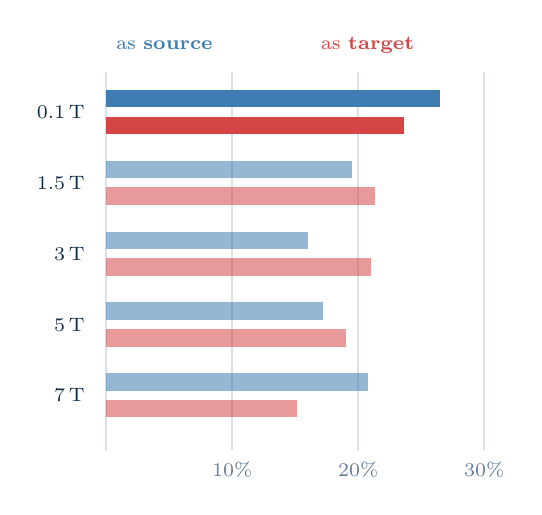
\begin{tikzpicture}[x=1cm,y=1cm,font=\scriptsize]
      \draw[draw=baseline,line width=0.8pt] (0,-0.3) -- (0,4.5);
      \foreach \x in {10,20,30}{
        \draw[draw=baseline,line width=0.6pt] (\x*0.16,-0.3) -- (\x*0.16,4.5);
        \node[text=muted] at (\x*0.16,-0.55) {\x\%};}
      % share of the total 1-SSIM error, as source (top bar) and as target (bottom bar)
      \foreach \y/\lab/\s/\t/\op in {%
        4.0/0.1\,T/26.5/23.6/1.0, 3.1/1.5\,T/19.5/21.3/0.55,
        2.2/3\,T/16.0/21.0/0.55, 1.3/5\,T/17.2/19.0/0.55, 0.4/7\,T/20.8/15.1/0.55}{
        \node[anchor=east,text=ink] at (-0.15,\y) {\lab};
        \fill[cond,opacity=\op]   (0,\y+0.06) rectangle (\s*0.16,\y+0.28);
        \fill[accent,opacity=\op] (0,\y-0.28) rectangle (\t*0.16,\y-0.06);}
      \node[text=cond,anchor=west,font=\scriptsize] at (0,4.85) {as \textbf{source}};
      \node[text=accent,anchor=west,font=\scriptsize] at (2.6,4.85) {as \textbf{target}};
    \end{tikzpicture}
  \end{column}

  \begin{column}{0.44\textwidth}
    \footnotesize
    \begin{itemize}\setlength{\itemsep}{2.2mm}
      \item 0.1\,T is \textbf{40\% of the transitions} and \hl{50\% of the error}.
      \item \emph{Toward} high field is easier than away from it: 7\,T the easiest
            target (0.9676), 3\,T the easiest source (0.9656).
      \item The model \textbf{adds} detail well and \textbf{removes} it badly.
    \end{itemize}
  \end{column}
  \end{columns}

  \srcline{Share of $\sum(1-\mathrm{SSIM})$ over 180 transitions, model \texttt{mc+ssim e8},
  scored locally. Each colour sums to 100\%.}
\end{frame}

% ================================================================ 5. the log
\begin{frame}{Every trial, one chart}
  \centering
  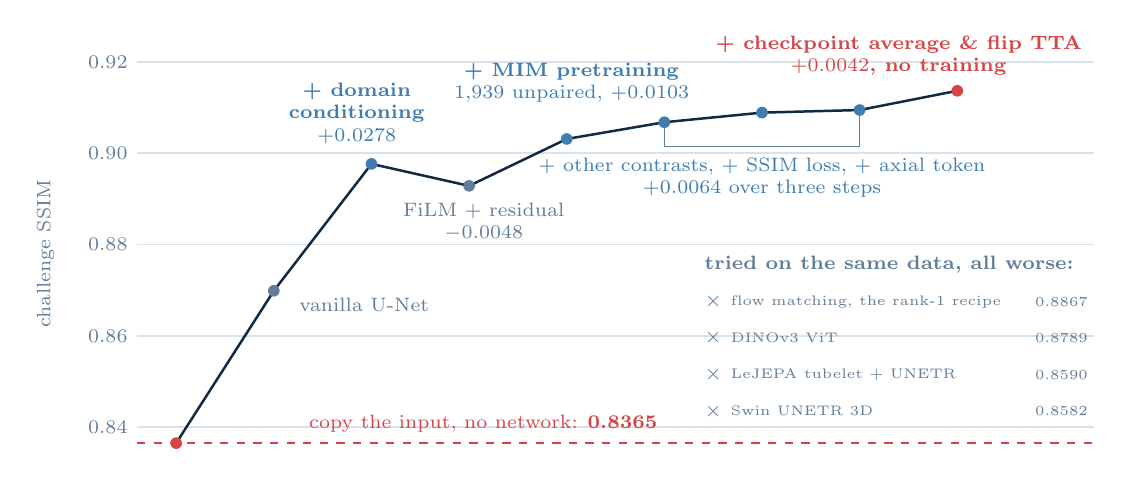
\begin{tikzpicture}[x=1.24cm,y=58cm,font=\scriptsize]
    % y is (challenge SSIM - 0.830); the whole frame spans 0.830 to 0.922.
    \foreach \v/\lab in {0.010/0.84,0.030/0.86,0.050/0.88,0.070/0.90,0.090/0.92}{
      \draw[draw=baseline,line width=0.6pt] (-0.4,\v) -- (9.4,\v);
      \node[text=muted,anchor=east,inner sep=1.5pt] at (-0.45,\v) {\lab};}
    \node[text=muted,rotate=90,anchor=south] at (-1.15,0.048) {challenge SSIM};

    % the identity control, as a floor under everything
    \draw[accent,dashed,line width=0.7pt] (-0.4,0.006497) -- (9.4,0.006497);
    \node[text=accent,anchor=west,inner sep=2pt] at (1.3,0.0108)
      {copy the input, no network: \textbf{0.8365}};

    % the spine, in build order
    \draw[ink,line width=0.9pt]
      (0,0.006497) -- (1,0.039856) -- (2,0.067646) -- (3,0.062839) --
      (4,0.073110) -- (5,0.076773) -- (6,0.078873) -- (7,0.079433) -- (8,0.083652);
    \foreach \x/\y/\c in {0/0.006497/accent, 1/0.039856/muted, 2/0.067646/cond,
                          3/0.062839/muted, 4/0.073110/cond, 5/0.076773/cond,
                          6/0.078873/cond, 7/0.079433/cond, 8/0.083652/accent}{
      \fill[\c] (\x,\y) circle (2.1pt);}

    % only the steps worth saying out loud; 5-7 are bracketed together
    \node[text=muted,anchor=west,inner sep=2pt] at (1.2,0.0368) {vanilla U-Net};
    \node[text=cond,anchor=south,align=center,inner sep=3pt] at (1.85,0.0702)
      {\textbf{+ domain}\\\textbf{conditioning}\\$+0.0278$};
    \node[text=muted,anchor=north,align=center,inner sep=2.5pt] at (3.15,0.0607)
      {FiLM $+$ residual\\$-0.0048$};
    \node[text=cond,anchor=south,align=center,inner sep=3pt] at (4.05,0.0792)
      {\textbf{+ MIM pretraining}\\1{,}939 unpaired, $+0.0103$};
    % one bracket for the three small information steps: labelling them apart costs more
    % room than they are worth at this scale.
    \draw[draw=muted,line width=0.5pt]
      (5,0.0757) -- (5,0.0715) -- (7,0.0715) -- (7,0.0783);
    \node[text=cond,anchor=north,align=center,inner sep=3pt] at (6,0.0709)
      {+ other contrasts, + SSIM loss, + axial token\\$+0.0064$ over three steps};
    \node[text=accent,anchor=south,align=center,inner sep=3pt] at (7.4,0.0851)
      {\textbf{+ checkpoint average \& flip TTA}\\\textbf{$+0.0042$, no training}};

    % everything tried on the same data that lost; the lower right is otherwise empty
    \node[text=muted,anchor=west,inner sep=2pt,font=\scriptsize] at (5.35,0.0455)
      {\textbf{tried on the same data, all worse:}};
    \foreach \y/\lab/\val in {0.0375/{flow matching, the rank-1 recipe}/0.8867,
                              0.0295/{DINOv3 ViT}/0.8789,
                              0.0215/{LeJEPA tubelet + UNETR}/0.8590,
                              0.0135/{Swin UNETR 3D}/0.8582}{
      \node[text=muted] at (5.5,\y) {$\times$};
      \node[text=muted,anchor=west,font=\tiny,inner sep=2pt] at (5.62,\y) {\lab};
      \node[text=muted,anchor=east,font=\tiny,inner sep=2pt] at (9.4,\y) {\val};}
  \end{tikzpicture}

  \vspace{0.5mm}
  \gloss{\info{Blue: information handed to the network.}
  \hl{Red: nothing added, just averaged.} Grey: architecture.}
\end{frame}

% ====================================================== 6. the decomposition
\begin{frame}{Where the 0.0772 came from}
  \centering
  \vspace{1mm}
  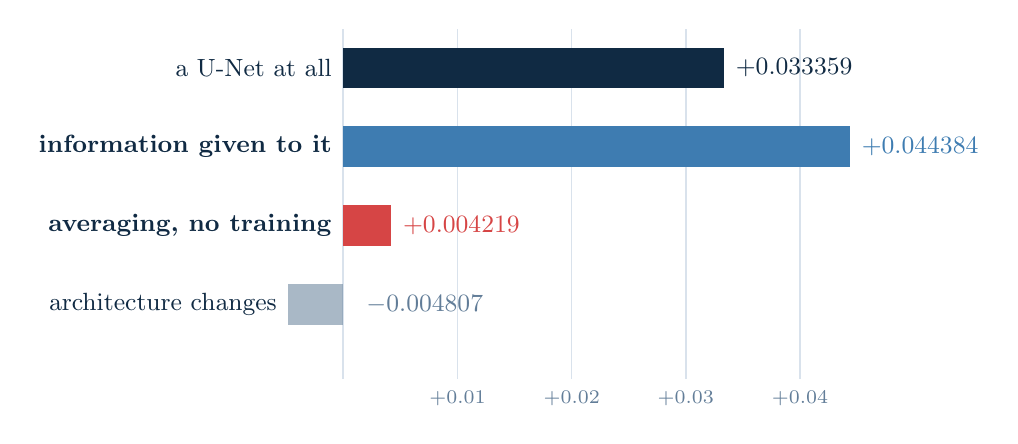
\begin{tikzpicture}[x=145cm,y=1cm,font=\small]
    \draw[draw=baseline,line width=0.7pt] (0,-0.55) -- (0,3.9);
    \foreach \v in {0.01,0.02,0.03,0.04}{
      \draw[draw=baseline,line width=0.5pt] (\v,-0.55) -- (\v,3.9);
      \node[text=muted,font=\scriptsize] at (\v,-0.8) {$+$\v};}

    \foreach \y/\lab/\val/\c in {%
      3.4/{a U-Net at all}/0.033359/ink,
      2.4/{\textbf{information given to it}}/0.044384/cond,
      1.4/{\textbf{averaging, no training}}/0.004219/accent}{
      \fill[\c] (0,\y-0.26) rectangle (\val,\y+0.26);
      \node[anchor=east,text=ink,inner sep=4pt] at (0,\y) {\lab};
      \node[anchor=west,text=\c,font=\small\bfseries,inner sep=4pt] at (\val,\y)
        {$+\val$};}

    % the one negative contribution, drawn the way it actually landed
    \fill[muted,opacity=0.55] (-0.004807,0.4-0.26) rectangle (0,0.4+0.26);
    \node[anchor=east,text=ink,inner sep=4pt] at (-0.004807,0.4) {architecture changes};
    \node[anchor=west,text=muted,font=\small\bfseries,inner sep=4pt] at (0.001,0.4)
      {$-0.004807$};
  \end{tikzpicture}

  \vspace{4mm}
  \gloss{$0.836497 \;\rightarrow\; 0.913652$. Four alternative backbones, same data,
  \textbf{every one} finished below the 32-channel U-Net.}
\end{frame}

% ============================================================ 7. qualitative
\begin{frame}{The two regimes, seen}
  \centering
  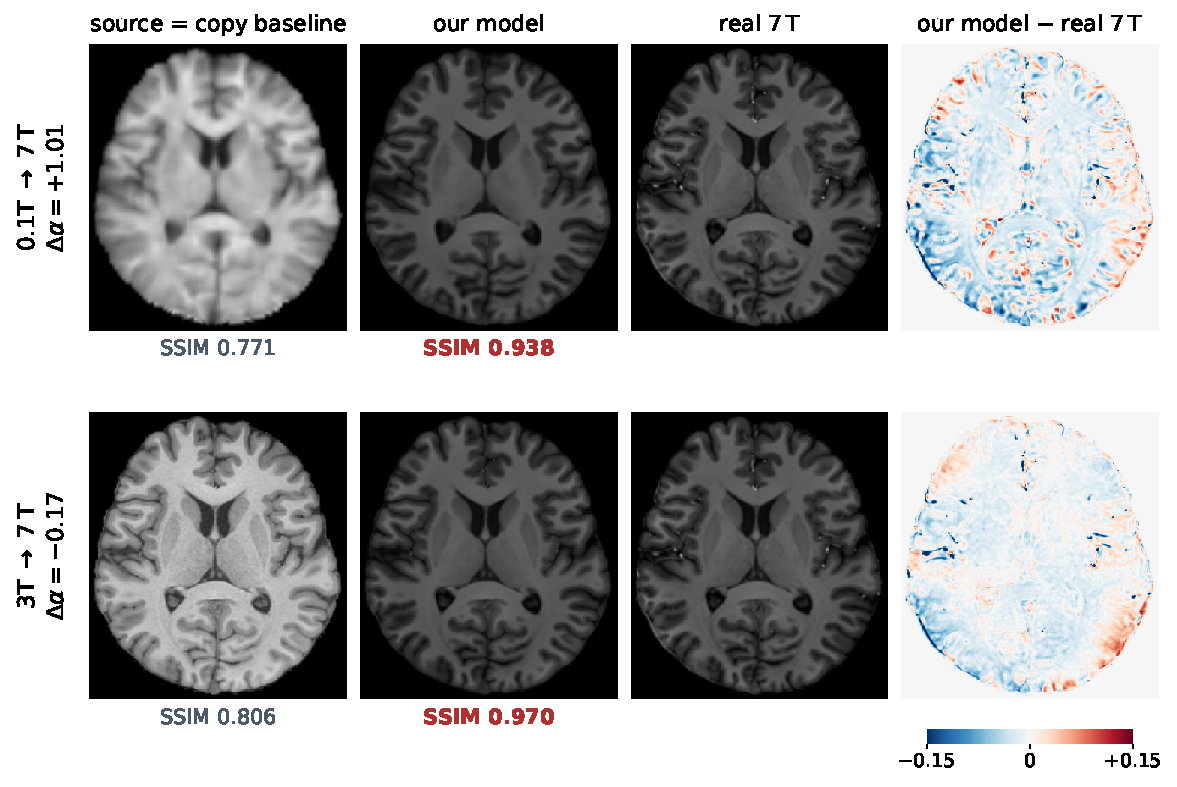
\includegraphics[height=0.78\textheight]{figures/slide_two_regimes.pdf}

  \vspace{0.5mm}
  \gloss{Residual is signed: \textcolor{cond}{blue $=$ too dark}, \hl{red $=$ too bright}.
  At 0.1\,T it piles up on the cortical ribbon; at 3\,T only on the outer rim.}
\end{frame}

% ================================================================= 8. closing
\begin{frame}{Taking it away}
  \vfill
  \begin{columns}[c,onlytextwidth]
  \begin{column}{0.46\textwidth}
    \centering
    \begin{tabular}{lr}
      \toprule
      \multicolumn{2}{c}{\textbf{Task 3 final}} \\
      \midrule
      SSIM   & \hl{0.913652} \\
      nRMSE  & 0.237970 \\
      LPIPS  & 0.090899 \\
      \bottomrule
    \end{tabular}

    \vspace{3mm}
    \gloss{32-channel conditional U-Net,\\ 4-channel input, MIM pretrained.}
  \end{column}
  \begin{column}{0.5\textwidth}
    \footnotesize
    \begin{enumerate}\setlength{\itemsep}{2.8mm}
      \item \textbf{Measure the gap before choosing a model.} The spectrum said two
        problems; the error map agreed; the backbone never mattered.
      \item \textbf{Pixel metrics are soft on blur.} The finest detail carries
        ${\sim}5\%$ of the variance the coarsest does.
      \item \textbf{Spend the last hour on averaging,} not on a new architecture.
    \end{enumerate}
  \end{column}
  \end{columns}
  \vfill
  \centering
  {\scriptsize\textcolor{muted}{Code, full architecture log and decision tree:
   \texttt{github.com/denizberkin/mrixfields-analysis}}}
\end{frame}

\end{document}
